% Chapter 6 is usually termed 'Evaluation' or 'Validation'. How did you test it? In which environment? How
% does it scale? Measurements, tests, screenshots. This chapter will have a volume of 10-15 percent of your
% thesis.
% In this chapter the implementation of Component X is evaluated. An example instance was
% created for every service. The following chapter validates the component implemented in
% the previous chapter against the requirements.
% Put some screenshots in this section! Map the requirements with your proposed solution.
% Compare it with related work. Why is your solution better than a concurrent approach from
% another organization?
% - compare the following approaches:
% suite.st
% http://www.eurofins-digitaltesting.com/test-tools/testwizard-automation-suite/

\chapter{Evaluation\label{cha:chapter6}}

Looking back to chapter \ref{cha:chapter3} describing the requirements of the final product we will evaluate the result and the usability of it in this chapter. The goal was to create a development and testing environment for HbbTV applications that is comparable with the state of the art of modern web development. Building web applications for the big screen turned out to be very cumbersome since there are no tools that help the developer to understand what is going on on the TV. Common workarounds are self build logging overlays on the developed application which might give information about certain variable states but don't disclose the insides of the app at all. The DevTools Backend component is the first tool that allows HbbTV developers to actually inspect a wide variety of aspects of an HbbTV application.

\begin{figure}[htb]
  \centering
  \hspace*{-0.7cm}
  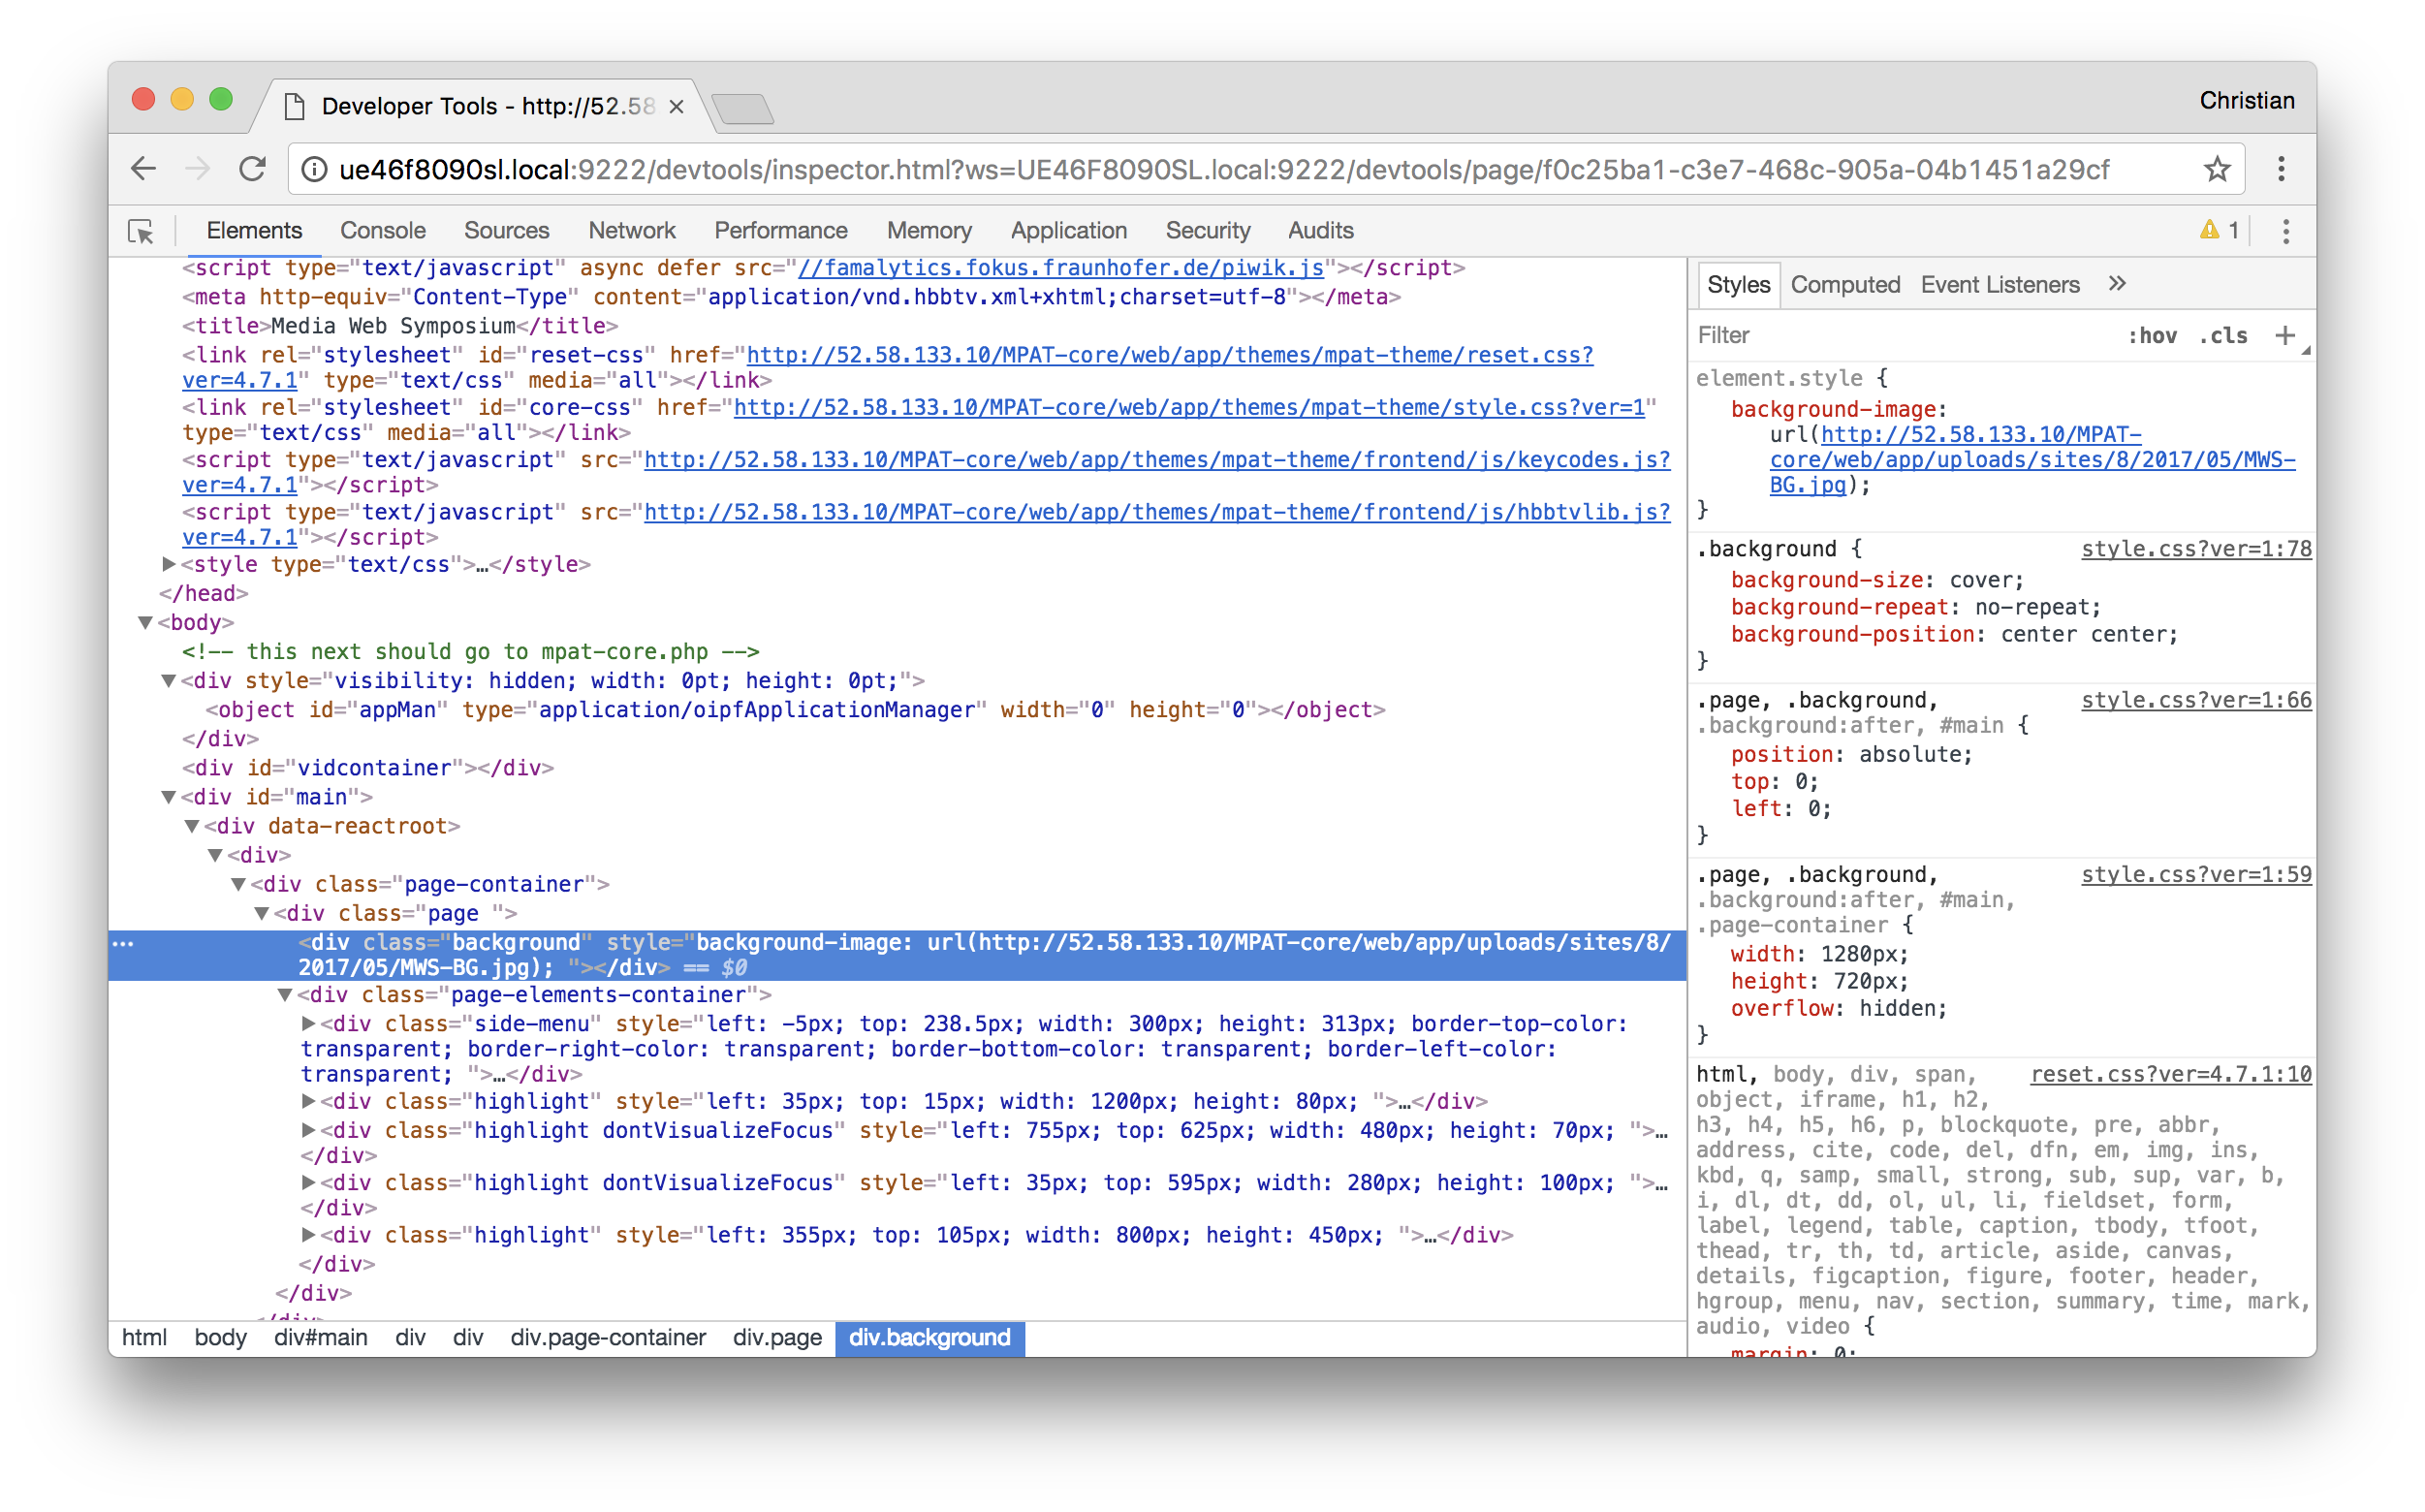
\includegraphics[width=16cm]{elementsPanel.png}\\
  \caption{Inspecting the DOM tree of an HbbTV Application using the DevTools application}\label{fig:elementsPanel}
\end{figure}

It not only allows to look into the DOM tree of the app but also to modify elements and their CSS properties. Developers have now the opportunity to build the app directly on the TV instead of having to implement it on a browser first and then test it on a real Smart TV. Instead of building a custom logging mechanism it automatically captures all logs from the page as well as JavaScript errors that were thrown. In addition to that the \textit{Console} tab of the DevTools application allows to execute any random JavaScript code within the context of the HbbTV page. With that it can inspect variables of your application during runtime. It can be used by the developer to see which JavaScript APIs are available in the browser environment of a specific target device.

\begin{figure}[htb]
  \centering
  \hspace*{-0.7cm}
  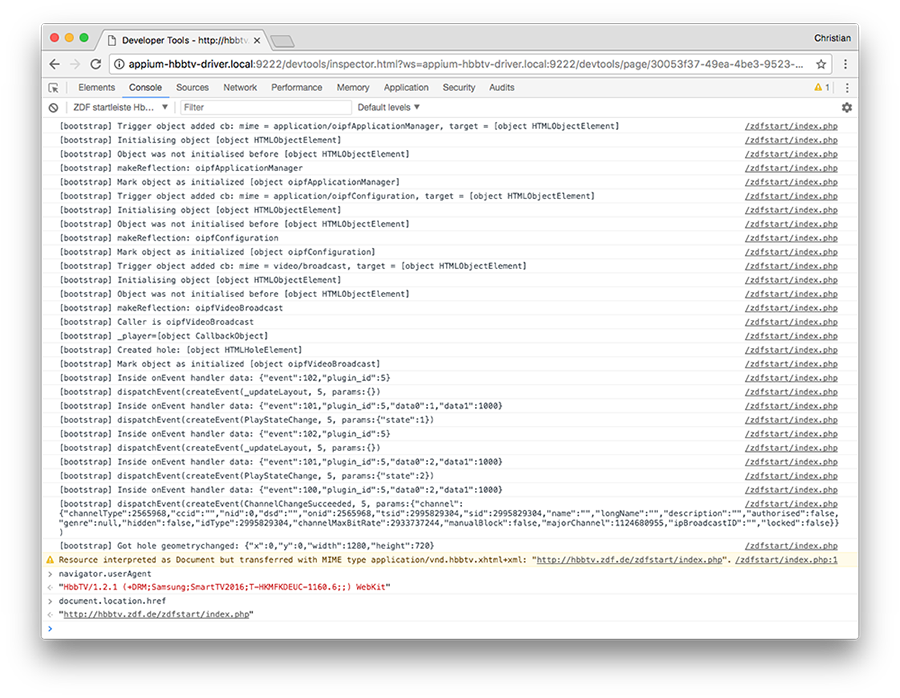
\includegraphics[width=16cm]{consolePanel.png}\\
  \caption{Debugging the ZDF HbbTV application with the Console tab}\label{fig:consolePanel}
\end{figure}

In addition to that since the TV is running all its network traffic through the proxy on the Raspberry Pi it automatically collects all network data in a way that it can be displayed in the DevTools application as well. It enables developers using this tool to not only see if all network requests have been resolved successfully on their own app but also on any arbitrary HbbTV applications that are published. This gives developers and researchers the chance to look into the loading behavior of an app to reveal information on when certain data is loaded and if the app is tracking the viewer behavior in any way. Like in the browser the DevTools application as seen in figure \ref{fig:networkPanel} shows not only a list of all network requests that have been made by the app but also their content.

\begin{figure}[htb]
  \centering
  \hspace*{-0.7cm}
  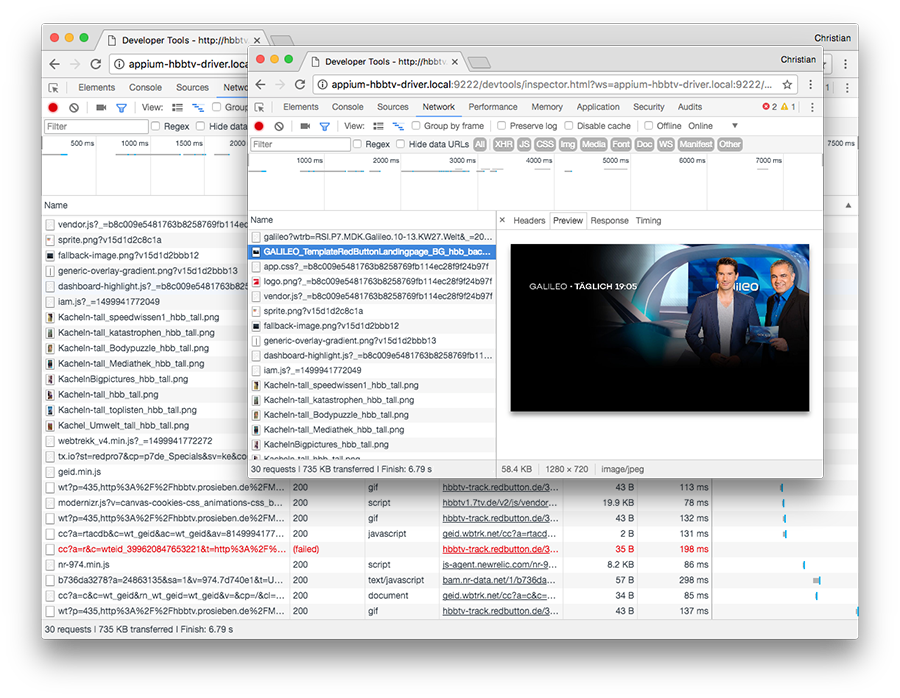
\includegraphics[width=16cm]{networkPanel.png}\\
  \caption{Network requests being made by the Pro7 HbbTV application}\label{fig:networkPanel}
\end{figure}

Sniffing through the requests shows that many small data packages that are covered as 1px gif images are sending user information to services like INFOnline\footnote{See request details in Annex section under listing \ref{ioam}} or a New Relic aggregator\footnote{See Annex section under listing \ref{newrelic}} containing data on the viewer origin, his TV, its model name and other device metrics. Another interesting artifact of data can be observed when switching around pages on the Pro7 HbbTV app. Every time a new page is opened a request is send to \url{hbbtv-track.redbutton.de} that tracks the movement of the viewer\footnote{Also shown in Annex section listing \ref{sniffing}}. After the application has fully loaded you can see at the bottom of the page that the main page took about 7 seconds to fully load and it downloaded 735 KB in 30 requests. This can be used to leverage interesting metrics of the performance of the HbbTV application.

Not only on the debugging side fulfills this tool all requirements that were stated before. Also its testing features raise above everything that has been done in the HbbTV industry before. Until now \textit{''most TV device browsers don’t support WebDriver''}\\ \cite{sengo}\footnote{The tool that is stated as HbbTV testing solution that supports Selenium doesn't exist anymore. There are no references on the internet other than this presentation.} but with the Appium HbbTV Driver developers can for the first time set up a grid of Smart TVs to run WebDriver tests on them. Since it is based on the WebDriver protocol which is the industry standard for automated desktop and mobile testing there are already hundreds of libraries available that can be used to write these automated tests. These libraries are available in all programming languages and flavors and already known by many developers that have experience with automated tests. As shown in listing \ref{lst:wdioExample} an automation script can be written within a couple lines of code. These tests are fairly simple to write even for non developers. There are solutions like Cucumber\footnote{\url{https://cucumber.io/}} that allow to abstract away the coding part of these tests by writing feature files with acceptance sentences which are translated into actual code. This makes writing e2e tests accessible for everyone.

\section{Automated HbbTV Test in CI/CD}

At the end of the thesis a project was setup that should simulate a continous delivery pipeline for a real HbbTV application. The goal was to setup an automated process that tests the app everytime a change was about to get introduced as e.g. a pull request in project that is managed with a version control system like Git\footnote{\url{https://git-scm.com/}}. For this reason a Jenkins server was setup in the TV lab at the Fraunhofer Fokus. Like in other common pipelines a job within Jenkins should get triggered once a patch was proposed to the project. Depending on the result of that test it should approve or reject the code change within the version control system. To accelerate the test execution a Selenium Grid server was setup to allow running tests in parallel on multiple TVs. Four different TV devices were equipped with a Raspberry Pi running the DevTools Backend and the Appium HbbTV Driver on them. All driver got registered to the grid server so that each test is properly directed to the right TV depending on its capabilities. For simplicity reasons the test project\footnote{\url{https://gitlab.fokus.fraunhofer.de/christian.bromann/mpat-webdriver-demo}} only contained the test files and not the app itself so that an already deployed HbbTV\footnote{The application to test here is the MPAT demo application of the Fraunhofer Fokus that is often to show off HbbTV demos at web media symposia. It can be found at \url{http://52.58.133.10/MPAT-core/web/mws/}} application can be used as guinea pig. To show that running functional tests with WebDriver is language agnostic the same test suite was written in 3 different programming language: Python, Ruby and Node.JS. It contained the following tests:

\noindent
\begin{table}[h!]
    \centering
    \begin{tabular}{|p{0.4\textwidth}|p{0.5\textwidth}|}
        \hline
        \textbf{Page} & \textbf{Tests} \\
        \hline
        Start &
        $\bullet$ should open correct page \newline
        $\bullet$ should collapse menu \vspace*{0.1cm} \\
        \hline
        Dynamic Ad-Insertion &
        $\bullet$ should open correct page \newline
        $\bullet$ should have a video element \\
        \hline
        DVB-T2 Broadcast Probing System &
        $\bullet$ should open correct page \newline
        $\bullet$ should not play video from the beginning \newline
        $\bullet$ should start the video \newline
        $\bullet$ should play video \\
        \hline
    \end{tabular}
    \caption{Test Scenarios for MPAT HbbTV App}
    \label{tab:table1}
\end{table}


\section{Comparison To Other Testing Solutions\label{sec:businessmodel}}

As of now there aren't any compatible testing solutions for HbbTV applications. The majority of developers still have to manually deploy their HbbTV applications on a server and setup a play out to access it on a real Smart TV device. However there is one company called Suitest that tries to simplify HbbTV testing with a click and play approach. It provides a service where developers can register their devices using a special hardware called Candy Box. The box is a \textit{''control unit which Suitest uses to operate TVs, Set-Top-Boxes and other devices through their infrared port''}\cite{candybox}. In combination with a paid subscription this box can be used to connect arbitrary devices with the Suitest cloud. The company allows then to signup on their website to create tests and manage accounts. As described in section \ref{sec:availabletestsolutions} the tests are being "clicked together" by a custom web interface where the developer can choose from a variety of action and assertion options. These tests can contain other tests which allows to split up multiple small tests to a big complex test suite. The concept of the service was patented in 2016 as an \textit{''invention [that] relates to a method and a system for testing interactive applications on at least one TV device (18) according to at least one test scenario''}\cite{krocek2016method}.

When signing up as a user at Suitest the first major difference immediately surfaces. The company provides their software as a service which means that it can only be used at higher scale by paying a monthly subscription. The test solution outlined in this thesis only requires hardware that costs once-only around 50\euro. The cheapest subscription plan at Suitest starts with 159\euro. There is also a free plan available to test the service. However this does not allow to run tests on a real Smart TV. In order to do that a Candy Box has to be purchased for 499\euro. Given that this box could instrument 40 devices the plan still doesn't allow to leverage the full potential of the Candy Box. Only with a paid subscription this box can be used properly.

The Candy Box itself is a useful piece of hardware that allows to instrument arbitrary TVs. Since it uses its infrared port it acts as remote control and has almost every ability to control the television like a human person. Connected to the internet and to the Suitest cloud every developer can control the TV using that box without having to be in the same location. The Raspberry on the contrary has certain limitations when it comes to controlling the TV. The instrumentation script of the DevTools Backend only works within a web environment. This means that the TV has to show an HbbTV app to allow the instrumentation script to work. This means that in order to run a test on the TV you need to turn it on and open an HbbTV application manually. Everything outside of the HbbTV context is not accessible. It is for instance not possible to open any internal menus or test a native application. These are indeed disadvantages against a box that uses an infrared connection to the TV. However looking at the scope of this thesis these limitations are acceptable. In addition to that the Raspberry Pi doesn't yet use any of the APIs that are provided by the manufacturer. Almost every TV can be accessed via an HTTP interface to gain control over certain features. These interfaces are used to allow mobile apps to work as e.g. a second remote control. Because the Pi is directly connected to the Smart TV, it has automatically access to these interfaces as well\footnote{As part of the research for this thesis a small Node.JS library (\url{https://gitlab.fokus.fraunhofer.de/christian.bromann/samsungtv}) was developed that can find and control newer Samsung Smart TV in the network by using its API interface.}. That being said, the way how the Candy Box can access the Smart TV can also be achieved using this approach.

Writing tests with the Suitest UI is fairly simple. As shown in figure \ref{fig:suitest} the UI provides an editor that allows to click together a chain of actions and assertions that can be read as normal English sentences. In order to choose elements from the app the developer can open up a utility menu that maps the mouse movements from the user to the app on the target device. Once the mouse hovers over an element it gets highlighted and can be chosen. In addition to that certain assertions, like the ''has property'' check, automatically fetch all available attributes the developer might be interested in. The editor in general feels slick and covers a variety of use cases that can ensure the expected state of the HbbTV application. Additional features like tagging or adding notes to certain steps are making tests not only easy to find but also easy to reason about. It doesn't require any technical experience to write, execute and maintain them. It is directed to not only app developers but also to project managers that want to make sure that certain requirements are met and features are implemented and stable.

The test environment developed with this thesis follows a completely different goal. It is based on already established industry standards like WebDriver and targets engineers directly. Tests are not "clicked together" using a GUI. They have to be written in a programming language and are usually created and maintained by the same developers that also build the HbbTV application. To interact with an element the selector has to be known. Since usually programmers are familiar with the elements on the page it is more difficult for other people, in or outside of the team, to write tests. However the DevTools Backend can give insights about the DOM structure of the application and allows to find these selectors. Still this approach requires some technical skills. The approach in general is non opinionated and allows to create custom delivery pipelines that is suited for any requirements a development team can have. While tests on the Suitest platform can only be scheduled in certain time intervals or on exact times, using the Appium HbbTV Driver it is possible to run tests at any desired point in time, e.g. when a certain release is being made or if new code is proposed and about to be merged into the code base. This allows creating gatekeepers that prevent bad code that causes regression to be introduced.

To summarize these points, the Suitest solution is a legitimized approach for quality assurance of HbbTV applications. The SaaS company sells a prescribed solution that is quite expensive though for a developer without much budget. The solution provided in this theses is build on top of established industry standards with proven success in other software markets. It is much more affordable and easier to integrate in common software pipelines. In long term has this approach a higher likelihood of being adapted in HbbTV developer workflows than the one provided by Suitest.

Even though their patent describes a similar approach to the one outlined in this thesis, it still doesn't violate their claims since all components are based on open standards and protocols. In fact their patent description explicitely talks about a \textit{''test scenario [that] is run and monitored by a test driver system separate from the at least one TV device''} \cite{krocek2016method} which describes a system that only purpose is to test an interactive application. The components developed in this thesis individually have a different purpose but can be setup in a way to achieve a similar goal. Important here is that the Appium HbbTV Driver can not only be used for testing, it is an instrument for automation in general. This is supported by the fact that the driver theoretically could also be used to automate any WebKit based browser not only televisions. Therefor non of the components sole function is to test an interactive application. There is no functionality in neither of them that would provide a testing mechanism. With that it is up to the person who uses the components whether to test something or to just run a set of automated steps on the TV. The focus here is on automation and not testing. This is a major differentiation.
